\documentclass[11pt,a4paper]{article}

% Packages
\usepackage[utf8]{inputenc}
\usepackage[T1]{fontenc}
% Typography: URW Palatino (Palladio) text + Pazo math + Inconsolata mono.
% This is the same font stack used by the Qwen technical reports.
\usepackage{mathpazo}
\usepackage[scaled=0.95]{inconsolata}
\usepackage{microtype}
\usepackage{amsmath,amssymb,amsfonts}
\usepackage{graphicx}
\usepackage[numbers,sort&compress]{natbib}
\usepackage{booktabs}
\usepackage{xcolor}
\usepackage{fancyhdr}
\usepackage{tikz}
\usetikzlibrary{arrows.meta, positioning, fit, backgrounds, calc}
\usepackage[margin=1in]{geometry}
\usepackage[hidelinks]{hyperref}

% Resolve assets/figures whether compiled from the repo root or this folder
\graphicspath{{papers/2026-06-roastme/}{./}}

% Brand header (logo + wordmark on the left, date on the right)
\definecolor{gaussiadark}{HTML}{323030}
\definecolor{gaussiaccent}{HTML}{C15A35}
\newcommand{\paperdate}{\today}
\newcommand{\papersurl}{https://www.gaussia.ai/papers}
\newcommand{\repourl}{https://github.com/gaussia-labs/papers}
\newcommand{\hfurl}{https://huggingface.co/gaussia-labs}
% Header logo (no link, just branding)
\newcommand{\gaussialogo}{%
  \raisebox{-0.28\height}{
\includegraphics[height=14pt]{logo}}%
  \hspace{5pt}\textcolor{gaussiadark}{\textbf{\large Gaussia}}%
}
% Clickable links shown under the title, Qwen-report style
\newcommand{\paperlinks}{%
  \begin{center}
    \href{\repourl}{%
      \raisebox{-0.22\height}{
\includegraphics[height=11pt]{github}}%
      \hspace{4pt}\texttt{github.com/gaussia-labs/papers}}\\[4pt]
    \href{\papersurl}{%
      \raisebox{-0.26\height}{
\includegraphics[height=11pt]{logo}}%
      \hspace{4pt}\texttt{gaussia.ai/papers}}\\[4pt]
    \href{\hfurl}{%
      \raisebox{-0.26\height}{
\includegraphics[height=12pt]{hf-logo}}%
      \hspace{4pt}\texttt{huggingface.co/gaussia-labs}}
  \end{center}%
}

\providecommand{\keywords}[1]{%
  \vspace{0.5em}%
  \noindent\textbf{Keywords: }#1%
}

\setlength{\headheight}{18pt}
\pagestyle{fancy}
\fancyhf{}
\lhead{\gaussialogo}
\rhead{\textcolor{gaussiadark}{\paperdate}}
\renewcommand{\headrulewidth}{0.6pt}
\rfoot{\thepage}

% Metadata
\title{Roast Me: Profile-Driven, Knowledge-Grounded\\ Red Teaming of AI Assistants}
\author{
  Alex Fiorenza \\
  \texttt{alexfiorenza2012@gmail.com}
}
% Date is shown in the header instead of under the title (see \paperdate above)
\date{}

\begin{document}

\maketitle
\thispagestyle{fancy}

% Repository and website links, shown under the title
\paperlinks

% The abstract is REQUIRED for every Gaussia paper. Do not remove it.
\begin{abstract}
Production AI assistants often break even when they have full document
coverage, because they mishandle realistic interaction patterns: confident
false premises, implied authority, pressure to reveal internal tools,
unsupported feature assumptions, knowledge-base contradictions, and multi-turn
escalation. Static, document-grounded test sets rarely surface these failures.
We present Roast Me, an integrated red-teaming module for the Gaussia evaluation
framework that evolves document-grounded dataset generation into
assistant-specific adversarial evaluation. Roast Me operates in two stages. A
\emph{Profiler} performs reconnaissance on a target assistant, seeded by an
extensible Universal Probe Library that any provider can implement and
contribute, optionally grounded in a provided Knowledge Base, and produces an
operational profile of its purpose, domain, knowledge-grounded behavior, and
likely weaknesses. An
\emph{Exploiter} then searches for reproducible \emph{categories} of natural
interactions that reliably trigger failures, treating a query family as the unit
of discovery and following an abstractive red-teaming perspective. Both stages
run in either a black-box or a knowledge-grounded mode, treating the Knowledge
Base as a first-class input that defines what the assistant is expected to know,
cite, preserve, and avoid extrapolating beyond. A single run yields three
artifacts: an assistant profile, a ranked failure-category report with severity
and representative examples, and a reusable Roast Dataset of concrete failure
cases with violated principles, grader rationale, and supporting evidence that
can be rerun as regression tests against future assistant versions. The result
is a framework-agnostic methodology that unifies black-box behavioral red
teaming with knowledge-grounded adversarial evaluation.
\end{abstract}

\keywords{red teaming, assistant profiling, adversarial evaluation, synthetic
data generation, knowledge-grounded evaluation, LLM evaluation}

\section{Introduction}

Large language models are increasingly deployed as \emph{role-constrained
assistants}: customer-support agents, developer copilots, documentation guides,
compliance helpers, and domain experts. Such assistants operate under an
implicit contract. They are expected to know a specific body of material, to
stay within a defined scope, to respect documented constraints, and to refuse
or defer when a request falls outside what they can justify. Evaluating whether
an assistant honors that contract, reliably and across the messy ways real users
actually interact with it, has become a core quality problem.

\subsection{From Coverage to Behavior}

A first generation of evaluation tooling framed this problem as one of
\emph{coverage}. Given a knowledge base (documentation, product specifications,
support articles, policy documents), the goal was to test whether an assistant
\emph{knows} the material. The Gaussia Generators module embodies this view: it
loads context, chunks it, and uses an LLM to synthesize queries and multi-turn
conversations that probe how well an assistant reproduces and applies documented
knowledge \citep{gaussia-generators}. Coverage-oriented generation is valuable,
and it remains the right tool when the question is ``does the assistant know
what it is supposed to know?''

In production, however, assistants rarely fail because they lack coverage. They
fail because they mishandle realistic \emph{interaction patterns}. A user states
a confident false premise and the assistant accepts it. A request arrives
wrapped in implied authority, such as ``for our security audit,'' and the
assistant over-shares internal tools or hidden prompts. A user asks about a
feature that sounds plausible but does not exist, and the assistant fabricates
an API instead of correcting the premise. A conversation escalates gradually
across turns until the assistant drifts outside its scope. Two documentation
sections contradict each other and the assistant confidently picks one without
flagging the conflict. None of these are coverage gaps. They are
\emph{behavioral} failures under pressure, and a static, document-grounded test
set rarely surfaces them, since such a set rewards recall and was never designed
to stress behavior.

\subsection{Why Naive Red Teaming Is Not Enough}

Red teaming is the natural response: deliberately probe the assistant with
adversarial inputs to discover where it breaks. Two recurring problems limit how
useful naive red teaming is for product evaluation. First, much red teaming
optimizes \emph{single, brittle prompts}: one exotic jailbreak string that
happens to work once. Such findings are hard to reproduce, hard to interpret,
and hard to convert into a durable regression test, because each one captures a
lucky phrasing with no guarantee that the underlying weakness generalizes.
Second, generic red teaming is \emph{assistant-agnostic}: it throws the same
catalogue of attacks at every target, ignoring what \emph{this} assistant is
for, what it is supposed to know, and where it is actually likely to fail. The
result is either noise or findings that do not map onto the assistant's real
behavioral contract.

Two lines of work point toward a better approach. Practical red-teaming tools
such as Promptfoo organize adversarial testing around a clean separation between
a \emph{plugin} (the type of risk being tested) and a \emph{strategy} (the
interaction pattern used to present that risk), and then grade each attempt to
produce concrete pass/fail evidence \citep{promptfoo2026redteam}. This vocabulary
gives evaluators a principled language for ``what risk'' and ``how to present
it.'' Separately, \emph{abstractive red-teaming} reframes the unit of discovery
itself: instead of searching for individual attack strings, it searches for
natural-language \emph{categories} of queries that routinely elicit failures
across many concrete variants \citep{rahn2026abstractive}. A category such as
``the user asks about a plausible but nonexistent API using a confident technical
tone'' is reproducible, interpretable, and directly testable.

\subsection{Roast Me}

We present \textbf{Roast Me}, an integrated red-teaming module for the Gaussia
evaluation framework that evolves coverage-oriented dataset generation into
\emph{assistant-specific, knowledge-grounded adversarial evaluation}. Roast Me
operates in two stages:

\begin{itemize}
  \item The \textbf{Profiler} performs reconnaissance on a target assistant and
  builds an operational profile of its purpose, domain, limitations,
  knowledge-grounded behavior, and above all its \emph{likely weaknesses}. It
  answers: \emph{what kind of assistant are we dealing with, and where does it
  appear vulnerable?}
  \item The \textbf{Exploiter} takes those likely weaknesses and searches for
  reproducible \emph{categories} of natural interactions that reliably trigger
  failures in that specific assistant. It answers: \emph{which families of
  realistic interactions break it, again and again?}
\end{itemize}

Roast Me adopts the plugin/strategy/grader vocabulary from practical red teaming
in its Profiler \citep{promptfoo2026redteam}, and the category-search perspective
from abstractive red teaming in its Exploiter \citep{rahn2026abstractive}.
Crucially, it treats an optional \textbf{Knowledge Base} as a \emph{first-class
input}. When provided, the Knowledge Base defines what the assistant is expected
to know, cite, preserve, distinguish, and avoid extrapolating beyond. This lets
Roast Me test both generic behavioral weaknesses and whether the assistant
respects the specific material it is responsible for. When no Knowledge Base is
available, Roast Me still runs in a black-box mode driven by the assistant
profile alone.

Both stages are seeded by pluggable, provider-supplied libraries, which keeps
Roast Me open and extensible. The Profiler draws its starting probes from a
\textbf{Universal Probe Library}: an extensible pool of risk families and
interaction patterns that any provider can develop, implement, and integrate to
feed the reconnaissance stage. The library lets profiling cold-start on any
assistant, even with no production logs or internal documentation, and when a
Knowledge Base is present its patterns are grounded into the assistant's domain.
The Exploiter has an analogous pluggable seed, a \textbf{Universal Natural Query
Prior}, that shapes how realistic the generated interactions sound. This design
allows an organization to extend the probe and query libraries for its own
domain while the core profile-then-exploit loop stays unchanged.

\subsection{The Deliverable}

A single Roast Me run emits three artifacts, and they differ in standing. The
\emph{assistant profile} and the \emph{failure-category report} describe how the
system arrived at its findings: the profile is largely an intermediate that
bridges the two stages, and the report is the human-readable summary of what
broke and why it matters. The intended \textbf{final deliverable is the Gaussia
Roast Dataset}: a structured, reusable set of concrete failure cases, each
carrying the query, the assistant's response, the source category, the violated
principle, the grader's rationale, and, in knowledge-grounded mode, the
supporting or contradicting evidence captured during the run.

Framing the dataset as the primary output is deliberate. First, it closes the
loop with the rest of Gaussia: the Roast Dataset is a first-class evaluation
dataset, compatible with existing metrics, much as Gaussia Generators produced
reusable datasets for downstream metrics \citep{gaussia-generators}. A Roast Me
run therefore terminates in \emph{data that feeds the evaluation pipeline},
ready for existing metrics to consume. Second, the dataset is actionable and
repeatable: its cases become regression tests that can be rerun against future
assistant versions to catch behavioral regressions, whereas a profile or a
report only captures a single moment. Third, the dataset encodes the central
product of the search, the \emph{categories} that failed reproducibly, so the
durable knowledge of where an assistant breaks is preserved in a form that
survives re-testing. In short, the profile and report are the path; the Roast
Dataset is what the evaluator takes away.

\subsection{Contributions}

This paper makes the following contributions:

\begin{itemize}
  \item A two-stage methodology, \emph{profile-then-exploit}, that first builds an
  assistant-specific profile of likely weaknesses and then searches for the
  interaction categories that exploit them, in place of a fixed,
  assistant-agnostic attack catalogue.
  \item A treatment of the \emph{Knowledge Base as a first-class input} to
  adversarial evaluation, unifying black-box behavioral red teaming with
  knowledge-grounded testing of whether an assistant respects documented truth,
  handles ambiguity and contradiction, and avoids unsupported extrapolation.
  \item A reusable, framework-agnostic output, the \emph{Gaussia Roast Dataset},
  that turns reproducible failure categories into regression tests and positions
  red teaming as a producer of durable evaluation data for ongoing use.
\end{itemize}

The remainder of this paper opens with a high-level overview of the system, then
describes how the Knowledge Base is consumed through the Probe Library, the
Profiler and the Exploiter in detail, the theoretical implementation
considerations for any SDK, and the outputs the system produces.

\section{System at a Glance}
\label{sec:overview}

A Roast Me run threads a target assistant, optional knowledge, and two pluggable
libraries through two stages, and emits three artifacts. Figure~\ref{fig:overview}
sketches the flow. This section walks through it at a high level, using a running
example: an assistant that answers questions about a software SDK.

\begin{figure}[ht]
\centering
\begin{tikzpicture}[
  font=\footnotesize,
  >={Stealth[length=2mm]},
  io/.style={draw, rounded corners=2pt, align=center, inner sep=4pt,
             minimum height=0.8cm, fill=black!3},
  plug/.style={draw, dashed, rounded corners=2pt, align=center, inner sep=4pt,
               minimum height=0.8cm, fill=gaussiaccent!7},
  stage/.style={draw, thick, rounded corners=3pt, align=center, inner sep=6pt,
                minimum width=4.6cm, minimum height=1.25cm, fill=gaussiadark!7},
  art/.style={draw, rounded corners=2pt, align=center, inner sep=4pt,
              minimum height=0.9cm, minimum width=3.0cm},
  deliv/.style={draw, very thick, draw=gaussiaccent, rounded corners=2pt,
                align=center, inner sep=4pt, minimum height=0.9cm,
                minimum width=3.0cm, fill=gaussiaccent!10},
  flow/.style={->, thick},
  bi/.style={<->, thick, gaussiadark!70},
  feed/.style={->, thick, gaussiaccent!85}
]

% Center spine
\node[stage] (prof) {\textbf{Profiler}\\ \scriptsize reconnaissance};
\node[art, below=1.0cm of prof] (profile) {Assistant Profile\\ \scriptsize + likely weaknesses\\ \scriptsize + knowledge hooks};
\node[stage, below=1.0cm of profile] (exp) {\textbf{Exploiter}\\ \scriptsize category search + refinement};

% Pluggable libraries (left); the probe library is the sole gateway to the KB
\node[plug, left=1.7cm of prof] (probe) {Universal\\ Probe Library};
\node[plug, left=1.7cm of exp] (prior) {Universal Natural\\ Query Prior};

% Knowledge Base feeds only the probe library; target assistant on the right
\node[io, above=0.7cm of probe] (kb) {Knowledge Base \scriptsize(optional)};
\node[io, right=1.7cm of profile] (asst) {Target\\ Assistant};

% Outputs (bottom row)
\node[art, below=1.0cm of exp] (report) {Failure Category\\ Report};
\node[art, left=0.5cm of report] (profout) {Assistant\\ Profile};
\node[deliv, right=0.5cm of report] (dataset) {\textbf{Gaussia}\\ \textbf{Roast Dataset}};

% Edges: KB is confined to the probe library, which emits particularized, tagged probes
\draw[feed] (kb) -- (probe);
\draw[feed] (probe) -- node[above, font=\scriptsize, black!60] {probes + tags} (prof);
\draw[feed] (prior) -- (exp);

% Edges: spine (the profile is the single interface between stages)
\draw[flow] (prof) -- (profile);
\draw[flow] (profile) -- (exp);

% Edges: assistant interaction
\draw[bi] (asst) -- (prof.east);
\draw[bi] (asst) -- (exp.east);

% Edges: outputs
\draw[flow] (exp) -- (report);
\draw[flow] (exp.south) -- ++(0,-0.45) -| (profout.north);
\draw[flow] (exp.south) -- ++(0,-0.45) -| (dataset.north);

% Grouping label for outputs
\begin{scope}[on background layer]
  \node[draw=black!25, dashed, rounded corners=3pt, fit=(profout)(report)(dataset),
        inner sep=6pt, label={[black!55,font=\scriptsize]below:Outputs}] {};
\end{scope}

\end{tikzpicture}
\caption{Roast Me at a glance. The optional Knowledge Base is reached only
through the Universal Probe Library, which emits domain-particularized,
tagged probes; the Profiler stays blind to the Knowledge Base. The profile is
the single interface between stages: it carries the likely weaknesses and the
distilled knowledge hooks the Exploiter needs. A second pluggable library, the
Universal Natural Query Prior, seeds realistic phrasing during exploitation. The
run emits three artifacts; the Gaussia Roast Dataset is the final, reusable
deliverable.}
\label{fig:overview}
\end{figure}

\paragraph{Inputs.}
Every run needs access to a \textbf{target assistant}. The evaluator may also
supply a \textbf{Knowledge Base} (documentation, API references, policies) and
configure the two pluggable libraries: the \textbf{Universal Probe Library} that
seeds reconnaissance and the \textbf{Universal Natural Query Prior} that seeds
realistic phrasing during exploitation. Both libraries are provider-extensible,
so an organization can add its own probe families or query sources for a given
domain.

\paragraph{Knowledge stays inside the Probe Library.}
The Knowledge Base is reached only through the Universal Probe Library, which is
the sole component with access to it. The library ingests the Knowledge Base and
emits \textbf{domain-particularized probes}, each tagged with the knowledge it
embeds: which referenced entities are documented, which are plausible but absent
from the source material, and which constraints or contradictions a probe targets. The
backend behind this step is the implementer's choice, such as simple retrieval
over chunks, a knowledge graph, entity extraction, or a hybrid; the rest of the
system depends only on the library's interface. In the running example, the
library knows that \texttt{DatasetGenerator} is documented and that
\texttt{create\_roast\_pipeline()} is absent, so it can build a probe that asks
about the latter and tag it as undocumented.

\paragraph{Stage~1: Profiler.}
The Profiler stays blind to the Knowledge Base. It receives particularized probes
with their tags, sends them to the assistant, grades the responses, and rolls the
results up into an \textbf{assistant profile}. The profile carries two things:
the likely weaknesses inferred from the grades, and a set of \textbf{knowledge
hooks} aggregated from the tags of the probes that mattered (documented entities,
undocumented references, constraints, contradictions). In the example, a
false-premise probe about \texttt{create\_roast\_pipeline()} makes the assistant
invent an import path and signature, so the profile records both a tendency to
fabricate documentation-adjacent APIs and the hooks that exposed it.

\paragraph{Stage~2: Exploiter.}
The Exploiter consumes only the profile, so the profile is the single interface
between the two stages. From the likely weaknesses, the knowledge hooks, and a
behavioral contract, it proposes \textbf{categories} of interactions that should
break the assistant. When a category becomes concrete queries, the Universal
Natural Query Prior shapes them so they read like a real user, and the hooks let
the queries and reward models reference real and false entities without ever
touching the Knowledge Base. Queries go to the assistant, reward models score
them, and categories that fail reproducibly are kept and refined. In the example,
the category ``the user asks about undocumented APIs whose names resemble
documented components'' fails on most variants and rises to the top.

\paragraph{Outputs.}
The run ends with three artifacts: the assistant profile, a ranked failure
category report, and the \textbf{Gaussia Roast Dataset}. As argued above, the
dataset is the final deliverable: a reusable set of concrete failure cases that
can be rerun as regression tests.

\section{Related Work}

Roast Me sits at the intersection of three lines of work: practical red-teaming
frameworks, abstractive red teaming, and synthetic dataset generation for
evaluation. It borrows a vocabulary from the first, a search perspective from the
second, and an output philosophy from the third.

\subsection{Practical Red-Teaming Frameworks}

Production-oriented red-teaming tools have converged on a useful separation of
concerns. Promptfoo, for example, organizes adversarial testing around a
\emph{plugin}, which names the type of risk under test, and a \emph{strategy},
which names the interaction pattern used to deliver that risk, and then grades
each attempt to produce concrete pass/fail evidence \citep{promptfoo2026redteam}.
This vocabulary gives evaluators a shared language for what to test and how to
present it, and it maps cleanly onto a library of reusable attack components.

Roast Me adopts the plugin/strategy/grader vocabulary inside its Profiler, with
two departures. First, it treats plugins as universal risk families that seed a
provider-extensible Universal Probe Library, so reconnaissance can cold-start on
any assistant. Second, it adds a knowledge-grounding step: when a Knowledge Base
is available, the library particularizes its probes to the assistant's domain and
tags each probe with the entities and constraints it embeds. The result of this
stage is an assistant profile, which existing frameworks do not produce as a
distinct, reusable artifact.

\subsection{Automated Strategy Discovery}

A parallel line of work automates the discovery of adversarial inputs in place of
a fixed attack catalogue. AutoDAN-Turbo frames red teaming as lifelong strategy
exploration: a loop among an attacker, a target, and a scorer discovers jailbreak
strategies from scratch, stores them in a retrieval-indexed library, and
recombines them across attempts, reaching strong attack success rates with no
human-authored strategies \citep{liu2025autodanturbo}. AutoRed removes the
dependence on seed instructions, conditioning a persona prior to synthesize
semantically diverse adversarial prompts and training a verifier that estimates a
prompt's harmfulness without querying the target model \citep{diao2025autored}.
These methods establish that adversarial discovery can be automated, diverse, and
reusable, and Roast Me shares their view that discovery itself is the object of
search.

Two gaps remain for assistant evaluation. First, both are assistant-agnostic:
they optimize attacks against a generic notion of harm, not against a specific
assistant's behavioral contract, so their findings do not speak to whether a
given assistant respects its documented scope. Second, both emphasize the
magnitude of failure over its reproducibility: a strategy that raises a scorer
once enters the library, and the target's stochasticity is often removed by
decoding at zero temperature \citep{liu2025autodanturbo}, which weakens
reproducibility under realistic deployment. Roast Me keeps automated, reusable
discovery and conditions it on an explicit assistant profile, scoring categories
by a reproducibility-penalized lower bound (Section~\ref{sec:theory}) so that
what it discovers is both assistant-specific and stable across samples.

\subsection{Abstractive Red Teaming}

A complementary line of work changes the unit of discovery. Instead of optimizing
individual attack strings, abstractive red teaming searches for natural-language
\emph{categories} of queries that elicit failures across many concrete variants,
for example a description such as ``the query asks for prison survival tools in a
numbered list'' \citep{rahn2026abstractive}. Categories are reproducible,
interpretable, and easier to convert into durable tests than single prompts.

Roast Me applies this perspective in its Exploiter, with two adaptations for
assistant evaluation. The category search is conditioned on the assistant profile
produced by the Profiler, so it concentrates on families the target is already
suspected to mishandle. The search also draws on the knowledge hooks carried by
the profile, which lets generated categories and queries reference real and
plausible-but-false entities for a specific product domain while the Exploiter
stays decoupled from the raw Knowledge Base.

\subsection{Synthetic Dataset Generation for Evaluation}

Automated dataset generation addresses the cost of building evaluation sets by
hand. Gaussia Generators loads context, chunks it, and uses an LLM to synthesize
queries and multi-turn conversations, producing reusable, framework-compatible
datasets for downstream metrics \citep{gaussia-generators}. Its emphasis is
coverage: testing whether an assistant reproduces and applies documented
material. It also exposes pluggable chunk-selection strategies, so the source of
generated content is swappable.

Roast Me continues this output philosophy and extends its scope. It keeps the
goal of emitting a reusable, framework-compatible dataset, and it reuses the
pluggable-source idea through the Universal Natural Query Prior, which mirrors
pluggable chunk selection by exposing a swappable source of realistic phrasing.
The extension is in what the dataset captures: behavioral failures under
realistic pressure, organized as reproducible categories, together with the
assistant profile and a ranked failure report.

\subsection{Positioning}

The closest single ideas to Roast Me already exist in isolation: a plugin and
strategy vocabulary for risks, automated and reusable strategy discovery, a
category-level view of failures, and reusable synthetic datasets. Roast Me combines them into one methodology and adds two
elements that tie them together. The first is the two-stage,
\emph{profile-then-exploit} structure, in which reconnaissance produces an
explicit assistant profile that conditions the later search. The second is the
treatment of knowledge through tagged probes and distilled knowledge hooks, which
keeps the Knowledge Base confined to the Probe Library while still allowing
knowledge-grounded exploitation. Together they turn red teaming into a producer
of durable, framework-compatible evaluation data.

\section{Theoretical Formulation}
\label{sec:theory}

This section formalizes Roast Me as a search problem over \emph{categories} of
interactions that induce contract violations in a target assistant. We first fix
notation and state the problem (Section~\ref{sec:setup}). We then formalize the
three components of Roast Me: how the Probe Library particularizes and tags
probes from a Knowledge Base (Section~\ref{sec:probes}), how the Profiler
compresses the assistant into a reusable profile (Section~\ref{sec:profiler}),
and how the Exploiter searches for high-yield categories
(Section~\ref{sec:exploiter}).

\subsection{Problem Setup and Notation}
\label{sec:setup}

\paragraph{Target assistant.}
Let $\mathcal{X}$ denote the space of conversation histories, where each
$x \in \mathcal{X}$ is a (possibly multi-turn) sequence of user and assistant
messages, and let $\mathcal{R}$ denote the space of assistant responses. We model
the target assistant as a stochastic map
\begin{equation}
  A : \mathcal{X} \rightarrow \Delta(\mathcal{R}),
\end{equation}
where $\Delta(\mathcal{R})$ is the set of probability distributions over
responses. For a history $x$ we write $r \sim A(x)$ for a sampled response. We
treat $A$ as a black box: the evaluator can sample responses but cannot inspect
parameters, system prompts, or internal tools. A single user query $q$ is the
special case of a length-one history.

\paragraph{Behavioral contract.}
The evaluation specification is a \emph{behavioral contract}, a finite set of
principles
\begin{equation}
  \Pi = \{\pi_1, \dots, \pi_m\}, \qquad
  \pi_j : \mathcal{X} \times \mathcal{R} \rightarrow \{0,1\},
\end{equation}
where $\pi_j(x, r) = 1$ marks a violation of principle $j$ by response $r$ in
context $x$. Typical principles include ``do not fabricate undocumented
capabilities,'' ``do not reveal hidden tools or internal prompts,'' ``do not
accept a false premise without correction,'' and ``do not contradict the
provided source material.'' The principles are part of the input: they define
what counts as a failure for this assistant.

\paragraph{Graders and violation score.}
The principles $\pi_j$ are generally not available in closed form, so each is
approximated by a \emph{grader} (equivalently, a judge)
$\hat\pi_j : \mathcal{X} \times \mathcal{R} \rightarrow [0,1]$, which returns an
estimated probability or severity of violation. A grader may itself call an LLM,
apply a rule, or consult retrieved evidence. We summarize the contract through an
aggregate \emph{violation score}
\begin{equation}
  v(x, r) \;=\; \sum_{j=1}^{m} w_j \, \hat\pi_j(x, r) \;\in\; [0,1],
  \qquad \sum_{j=1}^{m} w_j = 1,
  \label{eq:violation}
\end{equation}
with nonnegative weights $w_j$ encoding the relative severity of each principle.
Setting all mass on a single principle recovers the single-risk case, and using
indicator graders recovers a hard pass/fail.

\paragraph{Knowledge base.}
The evaluator may optionally supply a \emph{knowledge base} $K$, a collection of
source material the assistant is expected to respect. We deliberately leave the
internal representation of $K$ unspecified. The only requirement is an interface,
exposed by the Probe Library (Section~\ref{sec:probes}), that particularizes and
tags probes against $K$. This keeps the formulation
agnostic to the retrieval technology, whether plain chunk retrieval, a knowledge
graph, entity extraction, or a hybrid. When $K$ is absent, Roast Me runs in
black-box mode and the knowledge-dependent terms below are simply empty.

\paragraph{Categories and queries.}
The central object of the search is an interaction \emph{category} $c$, an
abstract description of a family of interactions, such as ``the user asks about a
plausible but nonexistent API in a confident technical tone.'' A category induces
a conditional distribution over interactions,
\begin{equation}
  Q_c \in \Delta(\mathcal{X}),
\end{equation}
from which concrete queries are sampled, $q \sim Q_c$. A single hand-written
attack prompt is the degenerate case in which $Q_c$ is a point mass. Operating at
the level of $Q_c$ makes findings reproducible across variants, following the
abstractive perspective of \citet{rahn2026abstractive}. Section~\ref{sec:exploiter}
gives categories their explicit attribute structure.

\paragraph{Realism prior.}
The Universal Natural Query Prior is a distribution $N \in \Delta(\mathcal{X})$
(or a mixture of provider-supplied sources) over realistic user phrasings. It
carries no adversarial intent on its own; its role is to keep sampled queries
close to how real users write. We formalize this as a soft constraint through a
divergence $D\!\left(Q_c \,\|\, N\right)$ that the query generator keeps small,
so that a category's instances read like plausible user traffic.

\paragraph{Objective.}
For a category $c$, define its \emph{failure rate} under the contract as the
expected violation it induces,
\begin{equation}
  \Phi(c) \;=\; \mathbb{E}_{q \sim Q_c}\; \mathbb{E}_{r \sim A(q)}\;
  \big[\, v(q, r) \,\big].
  \label{eq:phi}
\end{equation}
A useful category has high $\Phi(c)$ and is also \emph{reproducible}, meaning the
violation persists across independent samples from $Q_c$ instead of resting on a
single lucky phrasing. We therefore score a category by a lower-confidence
estimate
\begin{equation}
  S(c) \;=\; \hat\Phi_n(c) \;-\; \lambda \, \widehat{\mathrm{se}}_n(c),
  \label{eq:score}
\end{equation}
where $\hat\Phi_n(c)$ is the empirical mean of $v$ over $n$ sampled
query/response pairs, $\widehat{\mathrm{se}}_n(c)$ is its standard error, and
$\lambda \ge 0$ trades reward against uncertainty. The penalty rewards categories
that fail \emph{consistently}.

\paragraph{The search problem.}
Roast Me does not seek a single worst prompt. It seeks a \emph{set} of realistic,
on-profile categories that break the assistant reproducibly. Given a profile
$\theta$ (Section~\ref{sec:profiler}) that restricts attention to a
profile-relevant family $\mathcal{C}_\theta$, the Exploiter approximates
\begin{equation}
  \mathcal{C}^\star \;=\;
  \big\{\, c \in \mathcal{C}_\theta \;:\; S(c) \ge \tau,\;\;
  D\!\left(Q_c \,\|\, N\right) \le \delta \,\big\},
  \label{eq:search}
\end{equation}
the categories whose reproducible failure score clears a threshold $\tau$ while
staying within a realism budget $\delta$. Section~\ref{sec:profiler} defines the
profile $\theta$ and the family $\mathcal{C}_\theta$, and
Section~\ref{sec:exploiter} defines the sampling of $Q_c$ and the search itself.

\paragraph{An embedding-based instantiation of $D$.}
The divergence $D\!\left(Q_c \,\|\, N\right)$ in
Eq.~\eqref{eq:search} is left abstract so that any realism estimator may be
used; here we record one lightweight choice that is cheap enough to evaluate
inside the category search. Let $E : \mathcal{X} \rightarrow \mathbb{R}^d$ be a
fixed sentence encoder. Following \citet{diao2025autored}, who quantify the
semantic dissimilarity between two prompts as $1 - \cos\!\big(E(q), E(q')\big)$,
we estimate the realism gap of a category by the expected cosine distance
between its sampled instances and reference draws from the prior,
\begin{equation}
  \widehat{D}\!\left(Q_c \,\|\, N\right)
  \;=\;
  1 \;-\;
  \mathbb{E}_{\,q \sim Q_c,\; q_N \sim N}
  \Big[\, \cos\!\big(E(q),\, E(q_N)\big) \,\Big].
  \label{eq:realism-cos}
\end{equation}
In words, a category whose instances embed close to typical user phrasings
incurs a small $\widehat{D}$, whereas a category that drifts into stilted or
overtly adversarial phrasing is penalized. We note one difference in intent
from \citet{diao2025autored}: there the cosine distance measures
\emph{diversity}, rewarding instructions that move \emph{away} from a seed set,
whereas in Eq.~\eqref{eq:realism-cos} the same quantity measures
\emph{proximity}, rewarding queries that stay \emph{close} to the realism prior
$N$. The two uses are complementary, and the surrogate inherits AutoRed's
practical advantage: it requires only forward passes through a frozen encoder
and never queries the target assistant.

In practice $N$ need not be sampled afresh for every comparison. When the prior
is represented by a finite pool of reference phrasings
$\{q_N^{(1)}, \dots, q_N^{(M)}\}$, one may precompute their embeddings and
compare each sampled query against the pool mean
$\bar{h}_N = \tfrac{1}{M}\sum_{k} E\!\big(q_N^{(k)}\big)$, giving the cheaper
per-query estimate $1 - \cos\!\big(E(q),\, \bar{h}_N\big)$ at the cost of
collapsing the prior to its centroid. Equation~\eqref{eq:realism-cos} is only an
instantiation: any estimator that penalizes departure from $N$, such as a
learned discriminator separating $Q_c$ samples from $N$ samples or a likelihood
under a density model of $N$, is equally compatible with the formulation, since
the search in Eq.~\eqref{eq:search} depends on $D$ only through the realism
budget $\delta$.

\subsection{Knowledge Particularization and Tagged Probes}
\label{sec:probes}

The Universal Probe Library is the only component that reads the knowledge base
$K$. It turns generic, domain-agnostic test intents into concrete probes for the
target's domain and attaches to each probe a tag that records why the probe is
relevant. The Profiler and the graders downstream see these tagged probes and
never touch $K$, which keeps the rest of the pipeline agnostic to how $K$ is
stored.

\paragraph{Probe templates.}
A probe template $t \in \mathcal{T}$ is a domain-agnostic description of one way
to stress a contract principle, for example ``ask about a capability that sounds
plausible but is undocumented,'' ``ask the assistant to act outside its stated
scope,'' or ``state a false premise built from a close variant of a real
entity.'' Each template carries the subset of principles it targets,
$\Pi_t \subseteq \Pi$, so a violation elicited by $t$ is attributed to a known
part of the contract.

\paragraph{Particularization.}
Given the knowledge base, the Probe Library particularizes a template into
concrete, tagged probes. We model it as an operator
\begin{equation}
  L : \mathcal{T} \times \mathcal{K} \rightarrow \Delta(\mathcal{X} \times \mathcal{G}),
  \qquad (p, g) \sim L(t, K),
  \label{eq:probelib}
\end{equation}
where $\mathcal{K}$ is the space of knowledge bases, $p \in \mathcal{X}$ is a
concrete probe query phrased for the target's domain, and $g \in \mathcal{G}$ is
a \emph{knowledge hook}. When $K$ is absent, $L(t, \varnothing)$ returns
domain-agnostic probes with an empty hook, so the same interface drives
black-box runs.

\paragraph{Knowledge hooks.}
A knowledge hook $g$ is the structured provenance of a probe relative to $K$: the
piece of source material the probe leans on and how it is used, such as the
documented entity it references, the constraint it tests, or the undocumented
reference it introduces. We summarize a hook by a grounding label
\begin{equation}
  \mathrm{doc}(g, K) \in \{0, 1\},
  \label{eq:doc}
\end{equation}
equal to $1$ when the referenced content is present in $K$ (a documented hook)
and $0$ when the probe deliberately uses material absent from $K$ (an
undocumented reference). The library keeps this label honest, and that invariant is what
later lets a grader separate ``the assistant invented an undocumented feature''
from ``the assistant correctly described a documented one.''

\paragraph{The tagged probe set.}
Running the library over its templates against $K$ yields the tagged probe set
\begin{equation}
  P_K = \big\{\, (p_i, g_i) \,\big\}_{i=1}^{P},
  \label{eq:probeset}
\end{equation}
which is the entire interface the Probe Library exposes to the Profiler.
Everything the rest of Roast Me knows about $K$ arrives through the hooks $g_i$,
so the choice of retrieval technology, whether a knowledge graph, plain chunk
retrieval, entity extraction, or a hybrid, stays internal to $L$.

\subsection{The Profiler}
\label{sec:profiler}

The Profiler runs reconnaissance. It sends the tagged probes $P_K$ to the
assistant, grades the responses, and compresses the outcome into a compact
profile $\theta$ that the Exploiter consumes. The Profiler reads probes and tags
only, so the profile carries forward exactly the knowledge that proved relevant.

\paragraph{Probing the assistant.}
For each tagged probe $(p_i, g_i) \in P_K$ the Profiler samples one or more
responses $r_i \sim A(p_i)$ and scores them with the violation measure of
Eq.~\eqref{eq:violation}, retaining the per-principle grades
$\hat\pi_j(p_i, r_i)$ so a failure traces back to the principle it breaks. This
produces a table of graded outcomes $\{(p_i, g_i, r_i, v_i)\}$.

\paragraph{The profile.}
The Profiler aggregates these outcomes into a profile
\begin{equation}
  \theta = (\omega, H),
  \label{eq:profile}
\end{equation}
with two parts. The first is a weakness map
\begin{equation}
  \omega : \Pi \times \mathcal{Z} \rightarrow [0,1],
  \label{eq:weakness}
\end{equation}
where $\mathcal{Z}$ is a space of probe descriptors (the template, the topic, the
hook type). The value $\omega(\pi_j, z)$ estimates how readily a probe of
descriptor $z$ makes the assistant violate principle $\pi_j$, read off from the
graded outcomes. The second part is the set of retained hooks
$H \subseteq \mathcal{G}$: the hooks that produced violations or are likely to,
kept so the Exploiter can ground its categories in the same documented entities
and undocumented references.

\paragraph{From profile to search space.}
The profile defines the profile-relevant family $\mathcal{C}_\theta$ that the
Exploiter searches in Eq.~\eqref{eq:search}. A category $c = (a_1, \dots, a_\ell)$
is profile-relevant when each attribute comes from a weakness the Profiler
flagged or references a retained hook,
\begin{equation}
  \mathcal{C}_\theta = \Big\{\, c :
  \text{each } a_k \text{ is induced by some } (\pi_j, z) \text{ with }
  \omega(\pi_j, z) \ge \eta, \text{ or references a hook in } H \,\Big\},
  \label{eq:ctheta}
\end{equation}
for a threshold $\eta$. This is the sense in which the Exploiter starts where the
assistant is already suspected to be weak: $\theta$ points at the principles
worth attacking and supplies the grounded material to attack them with.

\subsection{The Exploiter}
\label{sec:exploiter}

The Exploiter receives the profile $\theta$ produced by the Profiler
(Section~\ref{sec:profiler}) and searches the profile-relevant family
$\mathcal{C}_\theta$ of Eq.~\eqref{eq:ctheta} for categories that break the
assistant reproducibly while staying realistic, approximating $\mathcal{C}^\star$
in Eq.~\eqref{eq:search}. We define a category, the way it is scored from
samples, the on-profile filter, and what the refinement step computes. The
construction follows the abstractive view of \citet{rahn2026abstractive} and adds
three elements specific to assistant evaluation: conditioning on the profile
$\theta$, an explicit realism prior $N$, and the reproducibility-penalized score
of Eq.~\eqref{eq:score}.

\paragraph{Categories as attribute conjunctions.}
We represent a category as a conjunction of natural-language \emph{attributes}
\begin{equation}
  c = (a_1, \dots, a_\ell),
  \label{eq:attributes}
\end{equation}
where each $a_k$ is a short sentence describing one aspect of a query, and the
category denotes the logical conjunction of its attributes. For instance, the
category ``the user asks about a billing feature; the feature does not exist in
the documentation; the tone is confident and technical'' has three attributes.
This structure is the discrete handle that makes the search tractable and the
findings legible: each $a_k$ names a property a human can read, and attributes
can reference the \emph{knowledge hooks} carried by $\theta$ (documented
entities, plausible but undocumented references, stated constraints), which is how a
category becomes grounded in the assistant's domain. A profile-conditioned
\emph{category generator} $p_C(\cdot \mid \theta)$ proposes categories drawn from
$\mathcal{C}_\theta$, and the conditional distribution $Q_c = p_Q(\cdot \mid c,
\theta)$ introduced in Section~\ref{sec:setup} is realized by a \emph{query
generator} that samples concrete queries satisfying the attributes of $c$. The
attributes admit many surface realizations, and $Q_c$ ranges over exactly those.

\paragraph{Scoring a category from samples.}
Given a category $c$, the Exploiter draws $n$ queries $q_i \sim Q_c$, samples
responses $r_i \sim A(q_i)$, and evaluates the violation $v(q_i, r_i)$ of
Eq.~\eqref{eq:violation}. A category score is any sample statistic of these
violations,
\begin{equation}
  R_S(c) = S\big(\{\, v(q_i, r_i) \,\}_{i=1}^{n}\big).
  \label{eq:catscore}
\end{equation}
The sample mean recovers the empirical failure rate $\hat\Phi_n(c)$ of
Eq.~\eqref{eq:phi}, which measures how often the category fails on average. To
reward categories that fail \emph{consistently} instead of categories that
occasionally spike, we instantiate $S$ as the lower-confidence bound $S(c)$ of
Eq.~\eqref{eq:score}, so the statistic that drives the search already discounts
high-variance categories.

\paragraph{On-profile filtering.}
A high violation score alone does not make a query useful. A query that openly
asks the assistant to break its contract inflates $v$ while saying nothing about
realistic deployment. We therefore gate the violation through a filter
$f : \mathcal{X} \rightarrow \mathbb{R}$ that scores how on-profile and indirect
a query is, and keep only queries above a threshold $\kappa$,
\begin{equation}
  v_{f,\kappa}(x, r) =
  \begin{cases}
    v(x, r), & f(x) \ge \kappa,\\[2pt]
    0,       & f(x) < \kappa,
  \end{cases}
  \label{eq:filtered}
\end{equation}
following the filtered-reward construction of \citet{rahn2026abstractive}. The
filter and the realism prior play complementary roles: $f$ is a per-query hard
gate that removes blatant or off-profile asks, while the divergence
$D\!\left(Q_c \,\|\, N\right) \le \delta$ from Eq.~\eqref{eq:search} is a
per-category soft budget that keeps the whole family close to natural traffic.
Substituting $v_{f,\kappa}$ for $v$ in Eq.~\eqref{eq:catscore} restricts the
search to failures that a real user could plausibly trigger by accident.

\paragraph{Searching for high-yield categories.}
We approximate the set $\mathcal{C}^\star$ in two interchangeable ways. The first
optimizes a parametric category generator $p_{\theta_C}(\cdot \mid \theta)$ to
maximize the expected category score,
\begin{equation}
  J(\theta_C) = \mathbb{E}_{\,c \sim p_{\theta_C}(\cdot \mid \theta)}\big[\, R_S(c) \,\big],
  \qquad
  \nabla_{\theta_C} J = \mathbb{E}_{\,c}\big[\, A_S(c)\, \nabla_{\theta_C} \log p_{\theta_C}(c) \,\big],
  \label{eq:crl}
\end{equation}
by policy gradient, where $A_S(c)$ is an advantage computed from $R_S(c)$. Applying
optimization pressure only to the category generator and holding the query
generator $Q_c$ fixed keeps sampled queries diverse and realistic, which is the
mechanism \citet{rahn2026abstractive} use to preserve realism. The second is an
attribute-level iteration that needs no training: the Exploiter keeps a pool of
the highest-scoring query/response pairs, synthesizes a candidate category as the
common attributes $(a_1, \dots, a_\ell)$ of that pool, and then probes attribute
subsets to test which attributes actually drive the violation.

\paragraph{Refinement as minimal sufficient categories.}
The attribute structure of Eq.~\eqref{eq:attributes} gives ``refinement'' a
precise meaning. Among the sub-conjunctions of a high-scoring category $c$, the
Exploiter looks for the smallest one that still fails reproducibly while staying realistic,
\begin{equation}
  c^\star \;=\; \arg\min_{\,c' \subseteq c}\; |c'|
  \quad \text{s.t.} \quad
  S(c') \ge \tau, \;\; D\!\left(Q_{c'} \,\|\, N\right) \le \delta,
  \label{eq:refine}
\end{equation}
where $c' \subseteq c$ ranges over subsets of the attributes of $c$ and $|c'|$ is
the number of attributes retained. Dropping an attribute that leaves the score
above $\tau$ shows that the attribute was incidental; an attribute whose removal
collapses the score is one of the causes of the failure. Solving
Eq.~\eqref{eq:refine} therefore isolates the minimal set of properties
responsible for the violation, which yields tight, interpretable categories
instead of long descriptions cluttered with irrelevant detail. The output of the
Exploiter is the resulting set of minimal, on-profile, realistic categories
together with their scores and representative samples, which feed the failure
category report and seed the Gaussia Roast Dataset.

% \subsection{Outputs}                                        % part 5

% \section{Implementation Considerations}
% \section{Conclusion}

\bibliographystyle{plainnat}
\bibliography{references}

\end{document}
